\section{Triển khai hệ thống}
Mục này đi sâu vào các khía cạnh kỹ thuật chính trong quá trình xây dựng và triển khai các thành phần của hệ thống VieVu. Quá trình này bao gồm việc chuyển đổi các thiết kế logic và kiến trúc thành mã nguồn hoạt động, thiết lập môi trường, tích hợp các công nghệ đã lựa chọn và xử lý dữ liệu cần thiết. Các nội dung chính được trình bày trong mục này bao gồm phương pháp thu thập và chuẩn bị dữ liệu ban đầu, chi tiết triển khai kỹ thuật cho các module AI cốt lõi (hệ thống tổng hợp tin nhắn và hệ thống gợi ý), và tổng quan về kiến trúc triển khai cuối cùng của toàn bộ hệ thống.

% \input{chapters/c4/system_design/4.1.1/4.1.1_video_design.tex}

% \input{chapters/c4/system_design/4.1.2/4.1.2_design_system.tex}

\subsection{Thu thập dữ liệu}


Để ứng dụng VieVu có thể hoạt động và cung cấp các chức năng cốt lõi như tìm kiếm, hiển thị thông tin, và gợi ý, việc xây dựng một bộ dữ liệu nền tảng ban đầu là bước thiết yếu. Dữ liệu ban đầu này bao gồm thông tin chi tiết về các địa điểm du lịch (attractions), các điểm đến lớn hơn (locations - tỉnh, quận,v.v.) và các loại hình du lịch (travel types).

\subsubsection{Nguồn và phương pháp thu thập dữ liệu}
Hệ thống thu thập dữ liệu từ hai nguồn chính là nền tảng \textbf{vn.trip.com} (cho dữ liệu chính về địa điểm, điểm đến, loại hình, và các thông tin khác) và \textbf{Ticketbox} (cho thông tin về các sự kiện).

Việc thu thập dữ liệu từ \texttt{vn.trip.com} gặp phải thách thức khi các yêu cầu truy cập trực tiếp bị chặn. Để giải quyết vấn đề này phải xây dựng một \textbf{proxy server bằng Node.js và TypeScript}. Proxy server này đóng vai trò trung gian, xử lý các yêu cầu đến \texttt{vn.trip.com} và cho phép việc thu thập dữ liệu diễn ra.

Trong quá trình thu thập, nhận thấy dữ liệu về mô tả (\texttt{description}) và phân loại loại hình du lịch (\texttt{travel\_type}) cho một số điểm tham quan bị thiếu hoặc chưa đầy đủ. Vì lý do này hệ thống đã tích hợp sử dụng \textbf{API của Google Gemini} để tự động tạo ra các mô tả và thông tin loại hình còn thiếu dựa trên thông tin có sẵn khác của điểm tham quan.

\subsubsection{Kết quả thu thập dữ liệu}
Thông qua quá trình crawling từ \texttt{vn.trip.com}, một bộ dữ liệu ban đầu đáng kể đã được thu thập và lưu trữ vào cơ sở dữ liệu PostgreSQL của hệ thống (quản lý bởi Supabase), bao gồm:
\begin{itemize}
    \item \textbf{1006 } bản ghi điểm tham quan (\texttt{attractions}), chứa các thông tin như tên, mô tả, ảnh bìa (\texttt{cover}), danh sách URL ảnh (\texttt{images}), điểm đánh giá (\texttt{hot\_score}, \texttt{avg\_rating}, \texttt{rating\_count}), giá tham khảo (\texttt{price}), tọa độ địa lý (\texttt{latitude}, \texttt{longitude}), địa chỉ (\texttt{address}), quy tắc giờ mở cửa (\texttt{open\_time\_rule}), và khóa ngoại liên kết đến địa điểm lớn (\texttt{location\_id}).
    \item \textbf{538} bản ghi điểm đến (\texttt{locations}), chủ yếu là các tỉnh/thành phố, quận của Việt Nam, chứa tên, ảnh, tọa độ và liên kết cha-con (nếu có).
    \item \textbf{100} bản ghi loại hình du lịch (\texttt{travel\_types}), bao gồm 12 loại hình cha và 88 loại hình con, lưu trữ dưới dạng ID (\texttt{id} dạng text) và tên (\texttt{name}).
    \item Bảng liên kết \textbf{\texttt{attraction\_types}} được tạo ra để quản lý mối quan hệ nhiều-nhiều giữa điểm tham quan và loại hình du lịch.
\end{itemize}
Các bảng này (\texttt{attractions}, \texttt{locations}, \texttt{travel\_types}, \texttt{attraction\_types}) được thiết kế với các khóa chính, khóa ngoại và chỉ mục (indexes) phù hợp như đã mô tả trong phần thiết kế CSDL (Mục \ref{sec:3-4-database}).

\subsubsection{Mục đích sử dụng dữ liệu}
Bộ dữ liệu được thu thập và làm giàu này đóng vai trò kép: (1) Cung cấp nội dung nền tảng phong phú cho các chức năng hiển thị, tra cứu, lọc thông tin địa điểm trên ứng dụng VieVu dành cho người dùng cuối. (2) Làm dữ liệu đầu vào quan trọng cho việc huấn luyện các mô hình gợi ý (recommendation models) sẽ được trình bày ở các mục sau.
Quá trình thu thập và chuẩn bị dữ liệu ban đầu này, dù gặp một số thách thức kỹ thuật, đã tạo ra nền tảng dữ liệu cần thiết cho sự hoạt động và phát triển của các tính năng cốt lõi trong hệ thống VieVu.



\subsection{Tổng hợp tin nhắn tạo lịch trình}
\label{subsec:summary_implementation_revised} % Label mới cho subsection

Một trong những tính năng ứng dụng AI nổi bật của VieVu là khả năng phân tích nội dung hội thoại trong nhóm chat và tự động đề xuất bản nháp lịch trình chi tiết cho chuyến đi. Để hiện thực hóa tính năng này một cách hiệu quả, tránh việc phải xử lý lại toàn bộ lịch sử trò chuyện mỗi khi người dùng yêu cầu, một kiến trúc xử lý gồm hai giai đoạn chính đã được thiết kế và triển khai trên nền tảng server FastAPI.

\subsubsection{Giai đoạn 1: Tiền xử lý Tin nhắn Bất đồng bộ}
\label{subsubsec:summary_phase1_revised}

Giai đoạn đầu tiên của pipeline tập trung vào việc xử lý các tin nhắn mới ngay khi chúng được gửi đến hệ thống, nhằm mục đích phân loại và trích xuất thông tin liên quan một cách tự động và bất đồng bộ.

Đầu tiên, để phát hiện tin nhắn mới một cách hiệu quả, hệ thống sử dụng cơ chế \textbf{LISTEN/NOTIFY} tích hợp sẵn của PostgreSQL. Một trigger cơ sở dữ liệu được cấu hình trên bảng \texttt{messages} để mỗi khi có một bản ghi mới được chèn, nó sẽ gửi một thông báo đến kênh \texttt{messages\_insert}, kèm theo dữ liệu (payload) của tin nhắn mới dưới dạng JSON, như minh họa trong Đoạn mã~\ref{lst:json-payload}. % (Xem chi tiết trigger tại Phụ lục \ref{apdx:db_trigger}) % <<< Placeholder

\lstset{language=json}
\begin{lstlisting}[
    caption=Payload JSON của tin nhắn mới (dạng dictionary Python),
    label=lst:json-payload,
    captionpos=t,
    belowcaptionskip=10pt,
    basicstyle=\small\ttfamily,
    breaklines=true,
    showstringspaces=false,
    inputencoding=utf8]
{
    "id": 335,
    "created_at": "2025-04-23T03:54:26.25777+00:00",
    "content": "Thu den Vinh Ha Long xem the nao cung duoc",
    "chat_id": 1,
    "meta_data": None,
    "is_travel_related": None,
    "chat_member_id": 10
}
\end{lstlisting}

\noindent Phía server FastAPI, một tác vụ nền \texttt{listen\_to\_messages} sử dụng thư viện \texttt{asyncio} của Python được khởi chạy và duy trì hoạt động liên tục nhờ cơ chế quản lý vòng đời \texttt{lifespan} của FastAPI. Tác vụ này thực hiện lệnh \texttt{LISTEN messages\_insert;} để lắng nghe các thông báo được gửi từ PostgreSQL trên kênh đã định. % (Xem mã nguồn hàm lắng nghe tại Đoạn mã \ref{lst:listener_code}) % <<< Placeholder

Tiếp theo là bước xử lý dữ liệu tin nhắn nhận được. Khi tác vụ nền nhận được dữ liệu payload của tin nhắn mới, nó thực hiện tuần tự các bước sau. Trước hết, nội dung tin nhắn được đưa vào hàm \texttt{classify\_sentence()} để thực hiện phân loại Zero-Shot  ZSC, sử dụng mô hình \texttt{joeddav/xlm-roberta-large-xnli} với hai nhãn \texttt{"travel schedule information"} và \texttt{"not travel schedule information"}. Kết quả phân loại, ví dụ như trong Đoạn mã~\ref{lst:zsc_output}, được dùng để xác định giá trị boolean \texttt{is\_travel\_related} dựa trên điểm tin cậy của nhãn \texttt{"travel schedule information"} $\geq 0.4$.

\lstset{language=json}
\begin{lstlisting}[
    caption=Output phân loại của mô hình ZSC (dạng dictionary Python),
    label=lst:zsc_output,
    captionpos=t,
    belowcaptionskip=10pt,
    basicstyle=\small\ttfamily,
    breaklines=true,
    showstringspaces=false,
    inputencoding=utf8]
{
    "sequence": "Thu den Vinh Ha Long xem the nao cung duoc",
    "labels": ["travel schedule information", "not travel schedule information"],
    "scores": [0.5240467190742493, 0.4759533107280731]
}
\end{lstlisting}

\noindent Nếu tin nhắn được xác định là liên quan (\texttt{is\_travel\_related = true}), bước nhận dạng tên địa điểm (NER) được thực hiện. Nội dung tin nhắn được xử lý bởi hàm \texttt{get\_place\_name()} (sử dụng thư viện \texttt{underthesea}). Các thực thể địa điểm mới tìm thấy, như minh họa trong kết quả tại Đoạn mã~\ref{lst:ner_output}, sẽ được định dạng và bổ sung vào trường \texttt{meta\_data} (JSONB) của tin nhắn, đồng thời tránh lưu trữ trùng lặp thông tin đã có.

\lstset{language=Python} % Giả định output này là tuple Python
\begin{lstlisting}[
    caption=Output nhận dạng thực thể của thư viện Underthesea,
    label=lst:ner_output,
    captionpos=t,
    belowcaptionskip=10pt,
    basicstyle=\small\ttfamily,
    breaklines=true,
    showstringspaces=false,
    inputencoding=utf8]
[
    ("Thu", "V", "B-VP", "O"),
    ("den", "E", "B-PP", "O"),
    ("Vinh", "N", "B-NP", "B-LOC"),
    ("Ha Long", "Np", "I-NP", "I-LOC"),
    ("xem", "V", "B-VP", "O"),
    ("the nao", "P", "B-NP", "O"),
    ("cung", "R", "O", "O"),
    ("duoc", "V", "B-VP", "O")
]
\end{lstlisting}

\noindent Sau đó, hệ thống áp dụng logic fallback để xử lý phản hồi khẳng định/phủ định. Cụ thể, nếu tin nhắn trước đó liên quan nhưng tin nhắn hiện tại không, hàm \texttt{classify\_affirmative()} (cũng dùng mô hình ZSC với các nhãn \texttt{"affirmation or negation"} và \texttt{"not affirmation and negation"}) sẽ kiểm tra xem đây có phải lời khẳng định/phủ định không. Nếu đúng, \texttt{is\_travel\_related} sẽ được đặt lại thành \texttt{true}. Cuối cùng, việc cập nhật cơ sở dữ liệu được thực hiện, lưu giá trị \texttt{is\_travel\_related} và trường \texttt{meta\_data} đã xử lý vào bản ghi tin nhắn tương ứng trong bảng \texttt{messages}. % (Xem chi tiết logic xử lý tại Đoạn mã \ref{lst:message_processing_logic}) % <<< Placeholder

Cuối cùng, trong Giai đoạn 1, hệ thống chuẩn bị thêm khâu xử lý dữ liệu tồn đọng. Để đảm bảo không bỏ sót tin nhắn gửi trong lúc server không hoạt động, hàm \texttt{update\_travel\_related\_status()} được thực thi khi server khởi động, thực hiện toàn bộ luồng xử lý ZSC, NER, Affirmation Check cho các tin nhắn có \texttt{is\_travel\_related} là NULL.

Kết thúc Giai đoạn 1, các tin nhắn trong cơ sở dữ liệu đã được phân loại và xử lý thông tin một cách tự động, tạo tiền đề dữ liệu cần thiết và tối ưu cho Giai đoạn 2.

\subsubsection{Giai đoạn 2: Tổng hợp và Tạo Lịch trình theo Yêu cầu}
\label{subsubsec:summary_phase2_revised}

Sau khi tin nhắn được tiền xử lý, Giai đoạn 2 được kích hoạt bởi người dùng để tạo bản nháp lịch trình cuối cùng, phối hợp giữa client (Flutter) và server (FastAPI).

Đầu tiên là bước chuẩn bị dữ liệu phía Client. Khi người dùng yêu cầu, ứng dụng Flutter truy vấn các tin nhắn liên quan mới nhất từ Supabase (đã được đánh dấu \texttt{is\_travel\_related=true}, mới hơn tin nhắn cuối được tổng hợp) kèm theo thông tin \texttt{message\_reactions}. Client tự xử lý logic vote từ reaction like/dislike để tạo marker `|Yes|` hoặc `|No|` nối vào cuối nội dung các tin nhắn tương ứng. Đồng thời, client thu thập metadata địa điểm, ngày đi và lịch trình cũ (nếu có).

Tiếp theo, client thực hiện gọi API tổng hợp phía Server. Client Flutter tạo JSON body chứa danh sách \texttt{conversation} (đã xử lý vote), \texttt{metadata}, \texttt{start\_date}, \texttt{end\_date}, và \texttt{previous\_summary} (nếu có), rồi gửi yêu cầu POST đến endpoint \texttt{/summarize} của server FastAPI cùng token xác thực. Cấu trúc JSON request hoàn chỉnh được minh họa trong Hình~\ref{fig:input}. % (Tham khảo mã gọi API tại Đoạn mã \ref{lst:client_api_call}) % <<< Placeholder
    \begin{figure}[H]
        \centering
        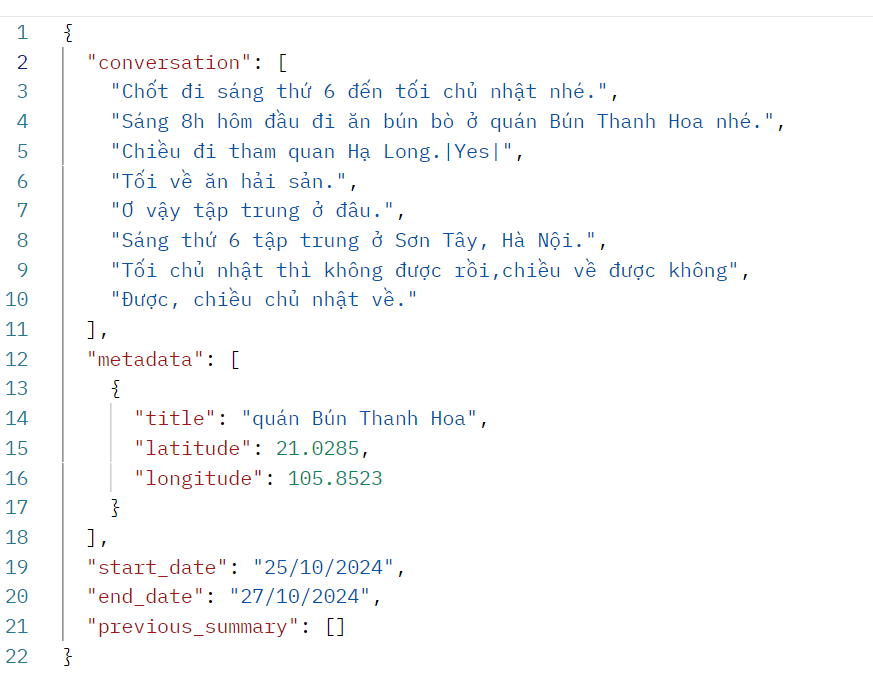
\includegraphics[width=0.8\textwidth]{figures/c4/input.png}
        \caption{JSON request hoàn chỉnh từ client gửi đến server.}
        \label{fig:input}
    \end{figure}

Sau đó, phía server thực hiện xây dựng Prompt. Server FastAPI nhận yêu cầu, tổng hợp dữ liệu và xây dựng một prompt chi tiết cho Google Gemini API (model flash 2.5), như minh họa trong Hình~\ref{fig:prompt}. Prompt này chứa đầy đủ ngữ cảnh và các chỉ dẫn cụ thể về cách tạo lịch trình dạng JSON theo yêu cầu (lọc sự kiện, xử lý Yes/No, liên kết metadata, gộp lịch trình cũ, tuân thủ định dạng output, v.v.). % (Tham khảo cấu trúc prompt chi tiết tại Phụ lục \ref{apdx:gemini_prompt}) % <<< Placeholder
    \begin{figure}[H]
        \centering
        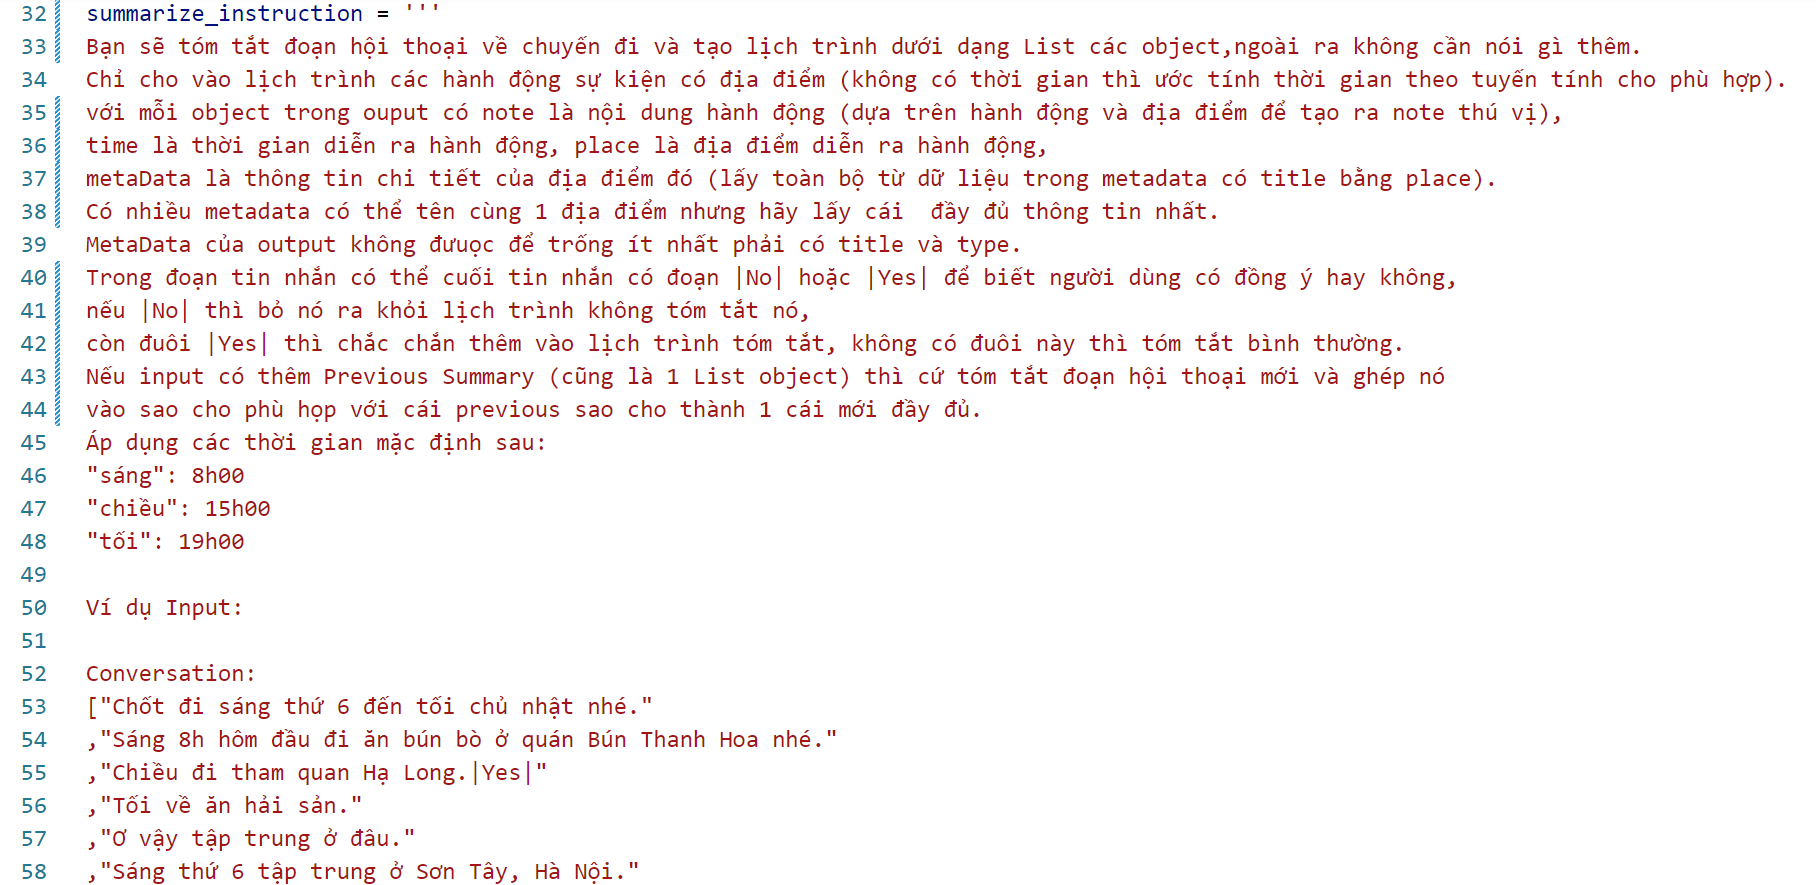
\includegraphics[width=0.9\textwidth]{figures/c4/prompt2.png}
        \caption{Prompt hướng dẫn Gemini tổng hợp lịch trình.}
        \label{fig:prompt}
    \end{figure}

Cuối cùng là bước xử lý kết quả, lưu trữ và phản hồi. Server FastAPI gửi prompt đến Gemini API, nhận phản hồi JSON chứa lịch trình, phân tích cú pháp kết quả đó. Sau đó, server thực hiện thao tác \texttt{upsert} vào bảng \texttt{chat\_summaries} để lưu/cập nhật lịch trình (\texttt{summary}), bản đọc (\texttt{readings}), và \texttt{last\_message\_id}. Kết quả lịch trình cuối cùng (ví dụ như trong Hình~\ref{fig:output}) được gửi về client Flutter để hiển thị.
    \begin{figure}[H]
        \centering
        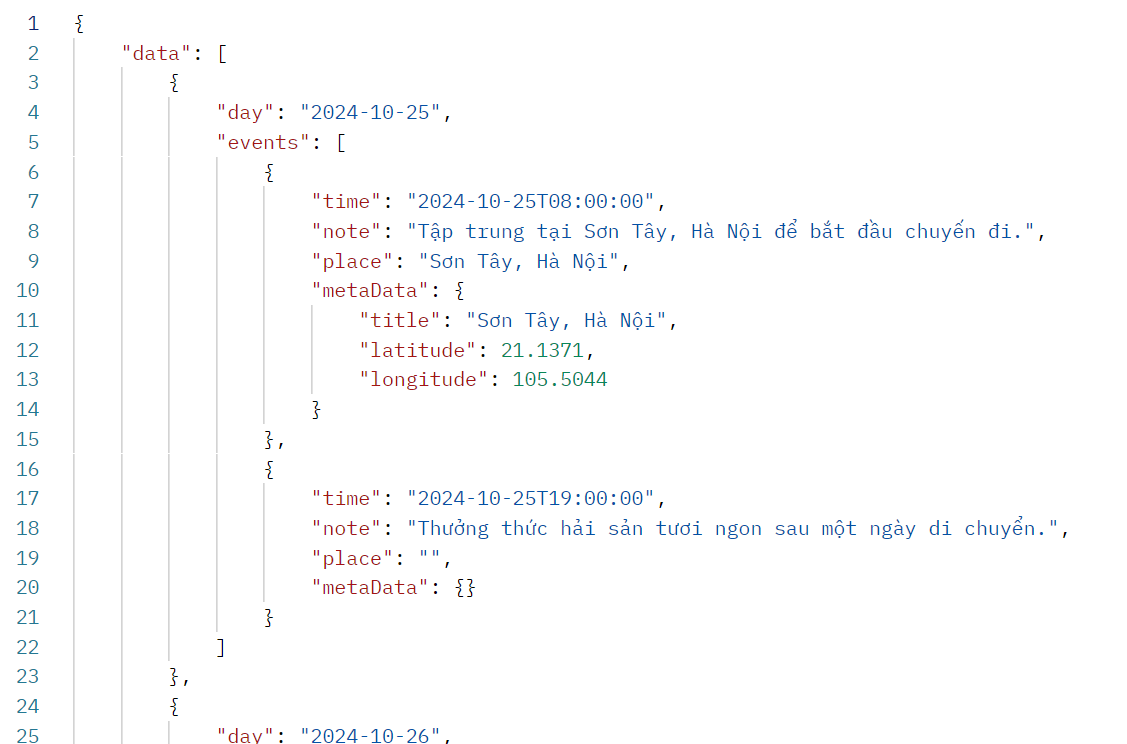
\includegraphics[width=0.8\textwidth]{figures/c4/output.png}
        \caption{Output JSON chứa lịch trình trả về từ server.}
        \label{fig:output}
    \end{figure}

Kiến trúc xử lý hai giai đoạn này, kết hợp tiền xử lý bất đồng bộ và tổng hợp thông minh theo yêu cầu bằng LLM, cho phép VieVu cung cấp tính năng hỗ trợ tạo lịch trình mạnh mẽ và hiệu quả.



\subsection{Triển khai Hệ thống Gợi ý}
\label{subsec:recsys_implementation_paragraph} % Label mới

Hệ thống VieVu triển khai hai cơ chế gợi ý chính để đề xuất địa điểm cho người dùng. Mục này trình bày chi tiết việc triển khai kỹ thuật cho cả hai cơ chế: gợi ý địa điểm liên quan dựa trên nội dung (Content-Based) và gợi ý địa điểm chính dựa trên Neural Network (Hybrid).

\subsubsection{Gợi ý Địa điểm Liên quan (Content-Based)}
\label{subsubsec:cb_recsys_impl_paragraph_final} % Label mới

Hệ thống gợi ý địa điểm liên quan hoạt động bằng cách kết hợp điểm đánh giá chất lượng/phổ biến nội tại của địa điểm với độ tương đồng về mặt nội dung văn bản. Đầu tiên, một điểm số nội tại ($Score_{Item}$) cho mỗi điểm tham quan được tính toán. Điểm này dựa trên điểm đánh giá trung bình có trọng số ($Score_{WeightedAvg}$) được làm mượt bằng công thức:
$$Score_{WeightedAvg} = \frac{R \times v + C \times m}{v + m}$$
Trong đó $R$ là điểm trung bình gốc, $v$ là số lượt đánh giá, $C$ là điểm trung bình toàn cục, và $m$ là ngưỡng tối thiểu. Sau đó, giá trị $Score_{WeightedAvg}$ và \texttt{hot\_score} được chuẩn hóa về thang [0, 1] ($ScaledWeightedAvg$, $ScaledHotScore$) và kết hợp thành $Score_{Item}$ cuối cùng với trọng số $w_{hs}=0.6, w_{wa}=0.4$:
$$Score_{Item} = w_{hs} \times ScaledHotScore + w_{wa} \times ScaledWeightedAvg$$
% (Tham khảo mã nguồn tại Đoạn mã \ref{lst:score_calculation}) % <<< Placeholder

Tiếp theo, nội dung văn bản của các địa điểm được tiền xử lý, tổng hợp thành trường \texttt{bag\_of\_words} và vector hóa bằng \texttt{TfidfVectorizer} từ Scikit-learn~\cite{sklearn_lib} (có loại bỏ từ dừng tiếng Việt) để tạo ma trận TF-IDF. Độ tương đồng nội dung giữa hai địa điểm (vector $\vec{a}$ và $\vec{b}$) được đo bằng Cosine Similarity:
$$\text{Cosine Similarity}(\vec{a}, \vec{b}) = \frac{\vec{a} \cdot \vec{b}}{\|\vec{a}\| \|\vec{b}\|}$$
Kết quả là ma trận độ tương đồng \texttt{cos\_sim} giữa các cặp địa điểm. % (Tham khảo tại Đoạn mã \ref{lst:tfidf_cosine_code}) % <<< Placeholder

Cuối cùng, hàm gợi ý \texttt{get\_related\_attractions} được triển khai. Hàm này nhận ID địa điểm đang xem, lấy $Score_{Item}$ và độ tương đồng nội dung ($Similarity$) từ \texttt{cos\_sim}, rồi tính điểm gợi ý cuối cùng ($Score_{Final}$) bằng cách kết hợp chúng với trọng số $w_{sim}$ (ví dụ: 0.7):
$$Score_{Final} = w_{sim} \times Similarity + (1 - w_{sim}) \times Score_{Item}$$
Top N địa điểm có $Score_{Final}$ cao nhất (trừ địa điểm gốc) được trả về thông qua API endpoint của FastAPI. % (Tham khảo tại Đoạn mã \ref{lst:related_attractions_func}) % <<< Placeholder

\subsubsection{Gợi ý Địa điểm Chính (Neural Network - Hybrid)}
\label{subsubsec:nn_recsys_impl_paragraph_final} % Label mới

Hệ thống gợi ý chính của VieVu, nhằm đề xuất địa điểm cá nhân hóa, được xây dựng dựa trên mô hình Neural Network (NN) theo cách tiếp cận Hybrid, sử dụng thư viện TensorFlow và Keras~\cite{tensorflow_lib, keras_lib}. Mô hình này dự đoán mức độ phù hợp (rating dự đoán) dựa trên sự kết hợp của ba nguồn thông tin: đặc trưng người dùng (User Features từ khảo sát/hành vi), đặc trưng địa điểm (Item Features gồm thuộc tính số và OHE loại hình), và dữ liệu đánh giá giả lập.

Quá trình chuẩn bị dữ liệu bao gồm tải dữ liệu đặc trưng cho khoảng 3500 người dùng và 1006 địa điểm. Do hạn chế dữ liệu rating thực tế, bộ dữ liệu huấn luyện (\texttt{user\_ratings\_data.csv}) được tạo giả lập bằng cách phân phối ngẫu nhiên điểm rating cho cặp (user, item) dựa trên thống kê gốc (\texttt{avg\_rating}, \texttt{rating\_count}) của địa điểm. Dữ liệu đặc trưng và rating giả lập sau đó được kết hợp và chia thành tập huấn luyện (90%) và kiểm thử (10%).

Mô hình NN được thiết kế theo kiến trúc two-tower song song. Nhánh người dùng và nhánh địa điểm nhận đầu vào là các vector đặc trưng tương ứng, mỗi nhánh đi qua hai lớp Dense (128 và 64 nơ-ron, ReLU). Output từ hai nhánh được ghép nối (Concatenate), đi qua một lớp Dense (64 nơ-ron, ReLU) và lớp Dense output cuối cùng (1 nơ-ron, 'linear') để dự đoán rating. Chi tiết thiết lập các lớp mạng được thể hiện trong Đoạn mã~\ref{lst:nn_model}. % (Sơ đồ kiến trúc có thể xem tại Hình~\ref{fig:nn_arch}) % <<< Placeholder

\lstset{language=python}
\begin{lstlisting}[
    caption=Thiết lập các lớp chính của mô hình Neural Network,
    label=lst:nn_model,
    captionpos=t,
    belowcaptionskip=10pt,
    basicstyle=\small\ttfamily,
    breaklines=true,
    showstringspaces=false,
    inputencoding=utf8]
    # User branch
    user_layer = Dense(128, activation="relu")(input_user)
    user_layer = Dense(64, activation="relu")(user_layer)
    # Attraction branch
    attraction_layer = Dense(128, activation="relu")(input_attraction)
    attraction_layer = Dense(64, activation="relu")(attraction_layer)
    # Merge and predict
    merged = Concatenate()([user_layer, attraction_layer])
    merged = Dense(64, activation="relu")(merged)
    output = Dense(1, activation="linear")(merged)
    
\end{lstlisting}

Mô hình được huấn luyện để tối thiểu hóa Mean Squared Error (MSE) giữa rating dự đoán và rating giả lập, sử dụng optimizer Adam (learning rate 0.001) và theo dõi Mean Absolute Error (MAE). Quá trình huấn luyện diễn ra trong 30 epochs với batch size 32. Kết quả huấn luyện được trực quan hóa trong Hình~\ref{fig:mae} cho thấy mô hình học được từ dữ liệu (Loss và MAE đều giảm) và đạt MAE khoảng 0.64 trên tập kiểm chứng, mặc dù có dấu hiệu overfitting. Mô hình với trọng số tốt nhất được lưu lại. % <<< NHỚ THAY LABEL FIG ĐÚNG !!!
    \begin{figure}[H]
        \centering
        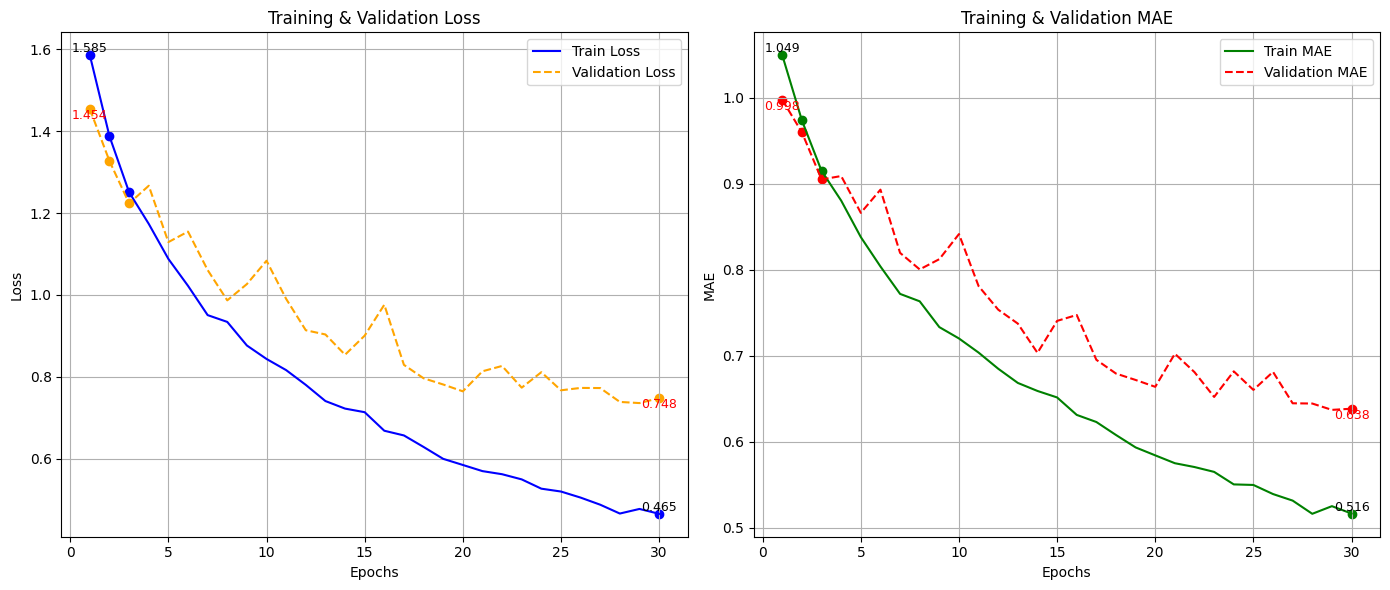
\includegraphics[width=\textwidth]{figures/c4/128.png} % Đường dẫn tới file ảnh của bạn
        \caption{Hiệu suất mô hình qua độ đo MAE và Loss trong quá trình huấn luyện.} % Cập nhật caption
        \label{fig:mae} % Giữ nguyên label nếu bạn đã dùng
    \end{figure}

Như vậy, việc triển khai hệ thống gợi ý địa điểm chính của VieVu đã hoàn thành thông qua việc xây dựng và huấn luyện mô hình Neural Network Hybrid. Bằng cách kết hợp thông tin đặc trưng và tín hiệu học hỏi từ dữ liệu rating giả lập, mô hình được tối ưu hóa để dự đoán mức độ phù hợp. Hệ thống gợi ý cuối cùng được tích hợp vào API server, sẵn sàng cung cấp các đề xuất địa điểm cá nhân hóa cho người dùng.


\subsection{Kiến trúc Hệ thống}
\label{subsec:system_architecture_impl}

Kiến trúc tổng thể của hệ thống VieVu khi triển khai là sự kết hợp giữa ứng dụng client (Flutter), nền tảng Backend as a Service (Supabase) và một backend tùy chỉnh (Python/FastAPI) cho các tác vụ chuyên biệt. Sơ đồ Hình~\ref{fig:system_architecture} minh họa các thành phần chính và luồng tương tác dữ liệu giữa chúng.

\begin{figure}[H]
    \centering
    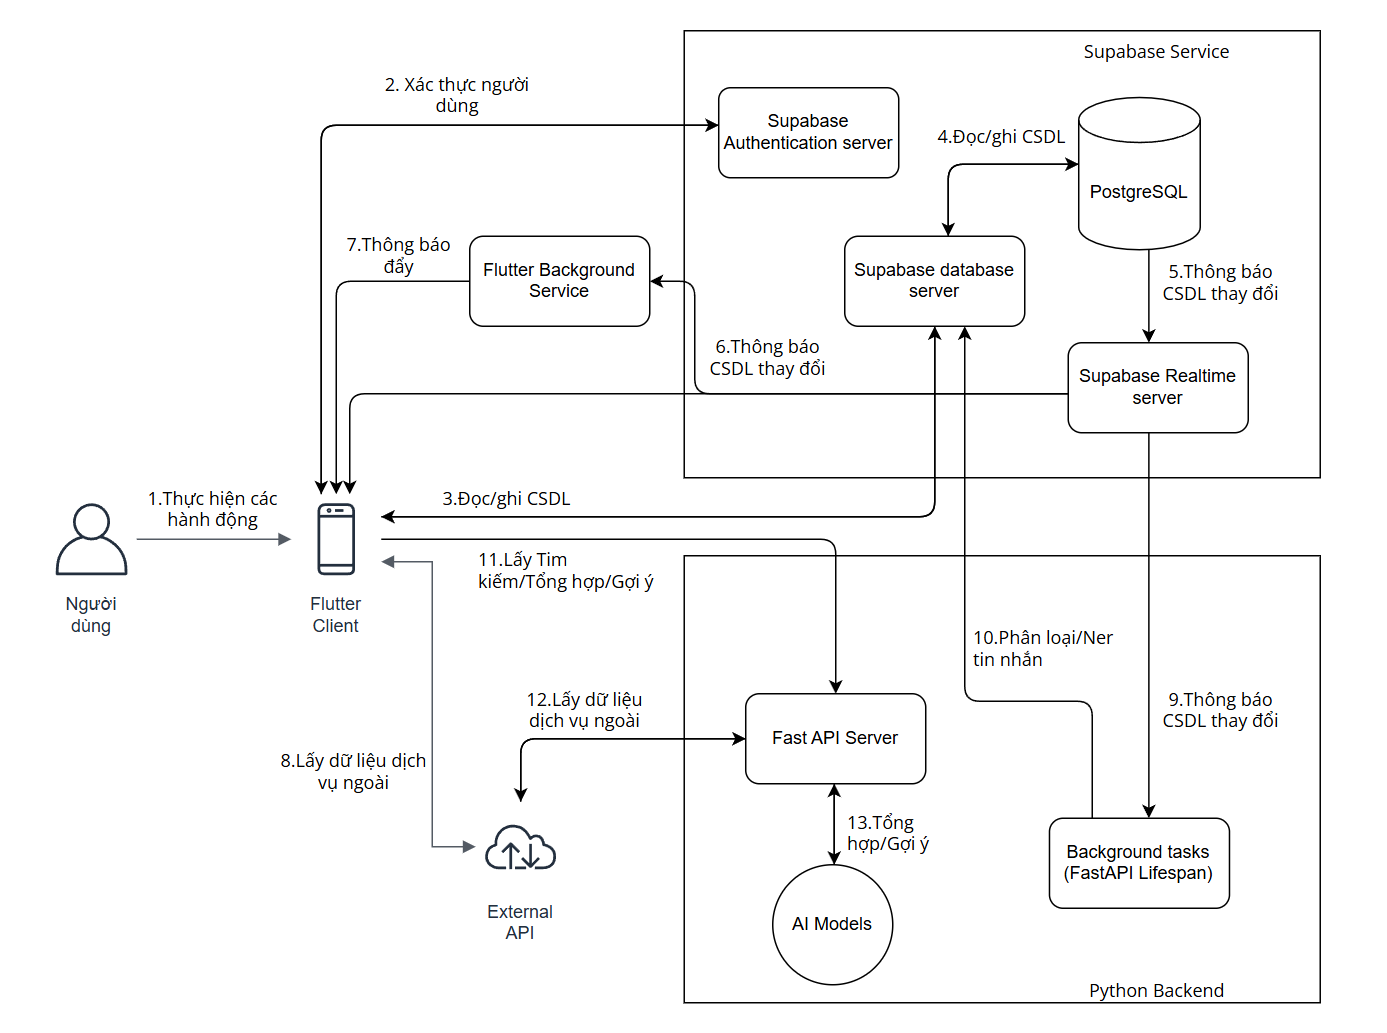
\includegraphics[width=1\textwidth]{figures/c4/architecture.png}
    \caption{Kiến trúc tổng thể của hệ thống VieVu.}
    \label{fig:system_architecture}
\end{figure}
\begin{enumerate}
    \item[-]\textbf{Người dùng (User):} Tác nhân chính tương tác với hệ thống thông qua ứng dụng client.
    \item[-]\textbf{Flutter Client:} Ứng dụng di động được xây dựng bằng Flutter, là giao diện chính để người dùng thực hiện các hành động như xem thông tin, lập kế hoạch, nhắn tin, yêu cầu gợi ý, v.v.
    \item[-]\textbf{Flutter Background Service:} Một dịch vụ chạy nền trên thiết bị người dùng (triển khai bằng Flutter), có thể dùng để xử lý thông báo hoặc đồng bộ dữ liệu nền tảng.
    \item[-]\textbf{Supabase Service:} Nền tảng BaaS cung cấp các dịch vụ backend cốt lõi, bao gồm:
        \begin{itemize}
            \item[-]\texttt{Supabase Authentication server:} Xử lý xác thực người dùng.
            \item[-]\texttt{Supabase database server:} Cung cấp API để tương tác trực tiếp với CSDL PostgreSQL.
            \item[-]\texttt{PostgreSQL Database:} Nơi lưu trữ dữ liệu chính của ứng dụng.
            \item[-]\texttt{Supabase Realtime server:} Quản lý các kết nối thời gian thực và phát các thay đổi dữ liệu.
        \end{itemize}
    \item[-]\textbf{Python Backend:} Backend tùy chỉnh được xây dựng để xử lý các tác vụ phức tạp, bao gồm:
        \begin{itemize}
            \item[-]\texttt{FastAPI Server:} Cung cấp các API endpoint cho các chức năng AI và tìm kiếm/tổng hợp.
            \item[-]\texttt{AI Models:} Các mô hình AI/ML đã huấn luyện (NN gợi ý, NER, ZSC,v.v.) được tải và sử dụng bởi FastAPI server.
            \item[-]\texttt{Background tasks (FastAPI Lifespan):} Tác vụ nền chạy bất đồng bộ bao gồm phân loại, nhận dạng tên, để tiền xử lý tin nhắn.
        \end{itemize}
    \item[-]\textbf{External API:} Các API của bên thứ ba (ví dụ: Trip.com, Ticketbox) mà Python Backend tương tác để lấy dữ liệu.
\end{enumerate}




\noindent Kiến trúc kết hợp này cho phép VieVu tận dụng các dịch vụ mạnh mẽ, sẵn có và khả năng mở rộng của Supabase cho các tác vụ phổ thông, đồng thời sử dụng một backend Python/FastAPI tùy chỉnh, linh hoạt để triển khai các thuật toán AI/ML phức tạp và tích hợp với các nguồn dữ liệu bên ngoài, tạo nên một hệ thống hoàn chỉnh và hiệu quả.

